\documentclass{article}

% Packages
\usepackage[utf8]{inputenc}
\usepackage{setspace}
\usepackage{titlesec}
\usepackage{fancyhdr}
\usepackage{lmodern}
\usepackage{amsmath, amssymb, geometry}
\usepackage{graphicx}
\usepackage{float}
\usepackage[hidelinks]{hyperref}

% Page setup
\renewcommand{\baselinestretch}{1.5}
\pagestyle{fancy}
\fancyhf{}
\fancyfoot[C]{\thepage}
\geometry{a4paper, margin=1in}
\renewcommand{\headrulewidth}{0pt}

\date{}

\begin{document}

% Title Page
\begin{titlepage}
\centering

\includegraphics[width=0.6\textwidth]{logoUSI.png}\\[1.5cm]

{\LARGE Università della Svizzera Italiana} \\[1.5em]
{\LARGE Faculty of Economics} \\[3em]

\vspace{1.5cm}

{\huge\bfseries Programming in Economics and Finance II} \\[2.5em]
{\LARGE\bfseries pyvar – A Python Package for Risk Management} \\[4.5em]

{\LARGE Alessandro Dodon, Niccolò Lecce, Marco Gasparetti} \\[3em]

{\LARGE\bfseries a.y. 2024/2025} \\[1.5em]
{\LARGE Submission Date: June 13, 2025} \\

\end{titlepage}


\tableofcontents
\clearpage % remove this to have introduction right after the ToC



\section{Introduction}

Risk management is central to finance, yet many practitioners still rely on inefficient tools like spreadsheets. As programming becomes essential in financial workflows, there is a growing need for accessible, efficient solutions to compute Value-at-Risk (VaR) and other risk metrics.

We introduce \texttt{pyvar}, a Python package that automates the full VaR estimation pipeline—from portfolio creation to risk metrics, visualization, backtesting, and natural language interpretation using LLMs. Focused on equity portfolios and simple models, the package prioritizes speed, clarity, and ease of use—ideal for both professionals and retail investors seeking intuitive, modern risk tools.


\section{Project Plan}

The project began with a presentation of our idea on April 16. Initially, we envisioned a minimal package focused on VaR, with core modules for normal parametric and historical VaR, simple volatility models, a Monte Carlo simulation module, basic backtesting via violation counting, and an interface for interaction with LLMs. Following a suggestion from our professor, we also added support for Expected Shortfall (ES), making the package more comprehensive and aligned with current risk management standards.

As development progressed—alongside our Risk Management course—we expanded the scope to include advanced volatility models, Extreme Value Theory, multivariate correlation structures, options-based P\&L modeling, factor models, and a complete suite of portfolio-level risk metrics.

Work was divided collaboratively. Alessandro Dodon implemented the volatility models, Extreme Value Theory, and backtesting routines. He also handled multivariate correlation modeling and portfolio risk decomposition. Marco Gasparetti developed the simulation modules (parametric and historical Monte Carlo), multi-day forecasting, and the options pricing framework. Niccolò Lecce integrated the large language model interface for natural language interpretation of results.

Factor models, extensive documentation and data download were jointly handled by Marco and Niccolò. All components were reviewed and tested as a team to ensure coherence and robustness.


\section{Project Diary}

Work on the project began after the idea was approved on the day of the presentation. Most of the initial development took place between April 17 and April 27 during the Easter break, following a kickoff meeting where tasks were divided.

We started by implementing the basic VaR models, volatility models, factor models, simulations, and LLM integration. More advanced components—such as improved backtesting, correlation modeling, options pricing, and enhanced visualizations—were added in the following weeks.

Weekly meetings, either in person or online, helped coordinate efforts and solve shared challenges. By early May, the core functionality was complete.

The final weeks were dedicated to refining code style, improving documentation, preparing examples, and assembling the full package.  
A detailed development history is available in our GitHub repository.


\section{Theoretical Foundation}

In this section, we present the mathematical foundations underlying each of our models. We begin with single-asset models, also referred to as univariate models, which focus on the return dynamics of a single asset or of a portfolio treated as a single aggregated position.

We then introduce a range of portfolio-level models, which explicitly consider the joint distribution of multiple asset returns. These include both analytical and simulation-based approaches. The section concludes with the backtesting methods used to evaluate the accuracy and reliability of our risk estimates.


\subsection{Basic VaR Models}

Value-at-Risk (VaR) at tail probability level $\alpha$ is defined as the smallest threshold $z_{\alpha}$ such that the probability of a loss exceeding it is $\alpha$. Equivalently, it is the $(1 - \alpha)$ quantile of the return distribution:
\[
\Pr\left(r_t < -z_{\alpha}\right) = \alpha.
\]
In monetary terms, this is typically scaled by \( W \), where \( W \) denotes the portfolio wealth. For simplicity, in single-asset models we omit \( W \) and use percentage-based notation.

We start with models that assume constant volatility over time. In the non-parametric (historical) approach:
\[
\mathrm{VaR}_{\alpha}^{\mathrm{hist}} = -\,\widehat{Q}_{\alpha}(r_t), \qquad
\mathrm{VaR}_{\alpha}^{\mathrm{normal}} = z_{\alpha} \sigma,
\]
and for portfolios this naturally extends to the normal parametric form. Expected Shortfall (ES), also known as Conditional VaR, is computed as:
\[
\begin{aligned}
\mathrm{ES}_{\mathrm{hist}} &= -\mathbb{E}\left[r_t \mid r_t < -z_{\alpha}\right], &
\mathrm{ES}_{\mathrm{normal}} &= \sigma \cdot \frac{\phi(z_{\alpha})}{\alpha}, &
\mathrm{ES}_{t_\nu} &= \sigma \cdot \frac{f_{t_\nu}(z_{\alpha})}{\alpha} \cdot \frac{\nu + z_{\alpha}^2}{\nu - 1},
\end{aligned}
\]
where $\phi$ is the standard normal density and $f_{t_\nu}$ is the density of the Student-$t$ distribution with $\nu$ degrees of freedom.

Normal and Student-$t$ VaR and ES estimates scale with the holding period as $\sqrt{h}$. For historical VaR, no scaling is needed—one can simply use weekly or monthly return data to estimate risk over longer horizons.


\subsection{Extreme Value Theory}


Technically still a parametric model, EVT is more sophisticated than the methods discussed above. We implement it with the Peaks-Over-Threshold (POT) approach: once a high threshold $u$ (e.g., the 99th-percentile loss) is chosen, a Generalized Pareto Distribution (GPD) is fitted to the excesses above $u$. 

VaR and ES are then derived analytically from the fitted GPD parameters. This allows for more accurate estimation of rare, extreme losses. The formulas used are:

\[
\begin{aligned}
{\text{VaR}}_\alpha &= u + \frac{\hat{\beta}}{\hat{\xi}}
\Bigl[\bigl(\tfrac{n}{n_u}(1-\alpha)\bigr)^{-\hat{\xi}} - 1\Bigr],\qquad
{\text{ES}}_\alpha &= \frac{{\text{VaR}}_\alpha + \hat{\beta} - \hat{\xi} u}{1 - \hat{\xi}},
\end{aligned}
\]

where $\hat{\xi}$ and $\hat{\beta}$ are the estimated shape and scale parameters, $n$ is the sample size, and $n_u$ is the number of exceedances.


\subsection{Volatility Models}

We have implemented the most popular univariate volatility models.

The GARCH(1,1) model is specified as:
\[
  \sigma_t^2 = \omega + a\, r_{t-1}^2 + b\, \sigma_{t-1}^2, \qquad r_t = \sigma_t z_t,
\]
where \( z_t \) are i.i.d.\ standardized shocks. VaR is then computed as:
\[
  \text{VaR}_{t,\alpha} = -\hat{\sigma}_t z_\alpha.
\]

Future volatility can be forecasted analytically using GARCH(1,1).

The \( \tau \)-step ahead forecast and cumulative \( T \)-step forecast are:
\begin{align*}
  \mathbb{E}[\sigma_{t+\tau}^2] &= \mathrm{VL} + (a + b)^\tau(\sigma_t^2 - \mathrm{VL}),  \\  
  \mathbb{E}[\sigma_{t,T}^2] &= \mathrm{VL}\left(T - 1 - \frac{(a + b)(1 - (a + b)^{T - 1})}{1 - (a + b)}\right)
    + \sigma_t^2\, \frac{1 - (a + b)^T}{1 - (a + b)},
\end{align*}
which naturally allow multi-period VaR estimation.

We also support EGARCH (logs variance, capturing leverage), GJR-GARCH (adds an indicator for negative shocks), and APARCH (introduces a power term for flexible tail dynamics), all with maximum-likelihood estimation under Normal, Student‐\( t \), GED, or Skew-\( t \) innovations.

For simpler benchmarks we include ARCH(\( p \)) and two rolling estimators, Moving Average (MA) and Exponentially Weighted Moving Average (EWMA):

\[
\sigma_{t}^{2,\mathrm{ARCH}}=\omega+\sum_{i=1}^{p} \alpha_{i}\, r_{t-i}^{2},\qquad
\sigma_{t}^{2,\mathrm{MA}}=\frac{1}{n}\sum_{i=1}^{n} r_{t-i}^{2},\qquad
\sigma_{t}^{2,\mathrm{EWMA}}=\lambda \sigma_{t-1}^{2}+(1-\lambda) r_{t-1}^{2}.
\]

ES for volatility models becomes:
\[
  \text{ES}_{t,\alpha} = -\hat{\sigma}_t \, \mathbb{E}[z_t \mid z_t < z_\alpha].
\] 

All our volatility models use a semi-empirical approach for the VaR computation, first calculating the empirical distribution of innovations with their respective volatility estimate and then using the required percentile of those innovations as \( z \).


\subsection{Time-Varying Correlation Models}

We now introduce models designed to capture time-varying correlations at the portfolio level, extending beyond single assets. Specifically, we implement two simple approaches: moving average (MA) and exponentially weighted moving average (EWMA), which mirror their univariate volatility counterparts.

Let \( x_t = (x_{1,t}, \dots, x_{N,t})^\top \) denote the vector of monetary positions, and let \( w_t = x_t / \sum_{i=1}^N x_{i,t} \) be the corresponding vector of portfolio weights. In this setting, we adopt both a parametric approach—assuming normally distributed returns—and a semi-empirical method based on standardized innovations.

VaR is computed as:
\[
\text{VaR}_t = z_\alpha \cdot \sqrt{w_t^\top \Sigma_t w_t},
\]
where \( \Sigma_t \) is the time-varying covariance matrix estimated by the model.

Expected Shortfall is computed either using the analytical formula under the normal distribution or with the semi-empirical method used for univariate volatility models.

More advanced multivariate models, such as DCC-GARCH or VEC(1,1), are not included due to limited support in Python.



\subsection{Factor Models}


We implement the Sharpe model and Fama-French three factor models to estimate portfolio VaR and ES. These models use asset betas with respect to systematic risk factors, allowing us to infer portfolio-level risk from exposures to common sources of variation.

For the Sharpe Model, we assume that each asset’s return $r_i$ follows the linear factor structure:
\[
r_i = \alpha_i + \beta_i r_m + \varepsilon_i,
\]
where $r_m$ is the return on the market portfolio, $\beta_i$ is the asset's sensitivity to the market factor, and $\varepsilon_i$ is a zero-mean idiosyncratic shock uncorrelated with $r_m$ and other residuals. The market return $r_m$ has variance $\sigma_m^2$, and $\mathrm{Var}(\varepsilon_i) = \sigma_{\varepsilon_i}^2$.

The total portfolio variance is:
\[
\sigma_p^2 = \left(\sum_{i=1}^N w_i \beta_i\right)^2 \sigma_m^2 + \sum_{i=1}^N w_i^2 \sigma_{\varepsilon_i}^2.
\]

VaR and ES are computed as follows under the normality assumption:
\[
\text{VaR}_{t,\alpha} = z_\alpha \cdot \sigma_p, \qquad
\text{ES}_{t,\alpha} = \sigma_p \cdot \frac{\phi(z_\alpha)}{1 - \alpha}.
\]
 
We also extend the previous model by considering three risk factors: market excess return (Mkt-RF), size (SMB), and value (HML). Each asset’s excess return is modeled as:
\[
r_i - r_f = \alpha_i + \beta_{i,1} \cdot \text{Mkt-RF} + \beta_{i,2} \cdot \text{SMB} + \beta_{i,3} \cdot \text{HML} + \varepsilon_i,
\]
where $r_f$ is the risk-free rate, and $\varepsilon_i$ is the idiosyncratic error. We estimate factor loadings $\beta_{i,k}$ through OLS regression.

Let $B$ be the $N \times 3$ matrix of estimated factor loadings, $\Sigma_f$ the $3 \times 3$ sample covariance matrix of the factors, and $\Sigma_\varepsilon$ the diagonal matrix of residual variances $\sigma_{\varepsilon_i}^2$. The total portfolio variance is:
\[
\sigma_p^2 = w^\top (B \Sigma_f B^\top + \Sigma_\varepsilon) w.
\]

Once the portfolio variance is known, we compute VaR and ES as we did for the single factor model.


\subsection{Analytic VaR}

We compute several Analytic VaR measures using the previously defined monetary position vector \( x_t = (x_{1,t}, \dots, x_{N,t})^\top \) and the covariance matrix \( \Sigma \). 

The quantile \( z_\alpha \) corresponds to the desired tail probability level and is always derived from the standard normal distribution, as the underlying assumption is that asset returns are normally distributed.

The asset-normal parametric portfolio VaR is defined as:
\[
  \text{VaR}_t = z_\alpha \cdot \sqrt{x_t^\top \Sigma x_t} \cdot \sqrt{h}.
\]

Assuming all asset returns are perfectly correlated (\( \rho = 1 \)) and there are no short positions, the undiversified portfolio VaR is simply the sum of the individual asset VaRs:
\[
  \text{UVaR}_t = \sum_{i=1}^N \text{VaR}_{i,t}.
\]

The marginal VaR, representing the sensitivity of portfolio VaR to a small change in position \( x_{i,t} \), is given by:
\[
  \Delta \text{VaR}_{i,t} = \text{VaR}_t \cdot \frac{(\Sigma x_t)_i}{x_t^\top \Sigma x_t}.
\]
It measures the change in total VaR from adding one extra unit of asset \( i \).

The component VaR is:
\[
  \text{CVaR}_{i,t} = x_{i,t} \cdot \Delta \text{VaR}_{i,t},
\]
which captures the absolute contribution of asset \( i \) to total portfolio VaR.

The relative component VaR is:
\[
  \text{RCVaR}_{i,t} = \frac{\text{CVaR}_{i,t}}{\text{VaR}_t},
\]
interpreted as the percentage share of total VaR attributable to asset \( i \).

For a vector \( a \) representing changes in the portfolio allocation, the incremental VaR is:
\[
  \text{IVaR}_t = \Delta \text{VaR}_t^\top \cdot a,
\]
which estimates the change in total VaR resulting from shifting the portfolio by \( a \).

Each of these VaR metrics can be complemented with a corresponding Expected Shortfall (ES), computed under the normality assumption.


\subsection{Simulation Methods}

Simulation methods are powerful tools for computing VaR and ES in portfolios that include complex instruments such as options, which exhibit non-linear payoffs.

We implement a one-day parametric Monte Carlo simulation approach under the assumption of multivariate normality. Future returns are simulated as:
\[
\mu = \mathbb{E}[r_t], \quad \Sigma = \operatorname{Cov}(r_t), \quad L = \operatorname{Cholesky}(\Sigma),
\]
\[
r^{(i)} = \mu + L z^{(i)}, \quad z^{(i)} \sim \mathcal{N}(0, I),
\]
\[
S^{(i)} = S_0 \circ (1 + r^{(i)}),
\]
where \( \circ \) denotes element-wise multiplication.

The simulated portfolio profit and loss is calculated as:
\[
\Delta P^{(i)} = w^\top(S^{(i)} - S_0) + \sum_{j=1}^{N_{\mathrm{opt}}} q_j \left(C(S_j^{(i)}, \tau_j') - C_{j,0}\right),
\]
where \( q_j \) is the number of option contracts, \( C(\cdot) \) is the Black-Scholes option price, and \( \tau_j' = \max(T_j - \tfrac{1}{252}, 0) \) is the adjusted time to maturity.

From the empirical distribution \( \{\Delta P^{(i)}\}_{i=1}^N \), we compute:
\[
\text{VaR}_\alpha = -\widehat{Q}_\alpha(\Delta P), \qquad
\text{ES}_\alpha = -\mathbb{E}[\Delta P \mid \Delta P \le -\text{VaR}_\alpha].
\]

We also implement a multi-day version of Monte Carlo, which forecasts VaR and ES over a longer horizon. This version is limited to pure equity portfolios.

As a non-parametric alternative, we implement Historical Simulation, both with and without replacement. We simulate alternative return paths by re-applying historical return vectors to the current portfolio. For each scenario \( i \), we define:
\[
S^{(i)} = S_0 \circ (1 + r_{\pi(i)}),
\]
where \( r_{\pi(i)} \) is the \( i \)-th sampled return vector, and \( \pi(i) \) is either the chronological index (historical simulation) or a random draw (bootstrap simulation).

The corresponding portfolio P\&L is:
\[
\Delta P^{(i)} = w^\top (S^{(i)} - S_0).
\]

Risk measures are computed as in the parametric case.

This approach is fully non-parametric and captures fat tails and nonlinear dependence in historical returns. When bootstrap is enabled, repeated resampling improves robustness in small-sample settings.


\subsection{Backtesting}


Backtesting assesses whether the observed losses are consistent with the VaR predictions by checking the frequency and structure of violations (exceptions). The objective is to test whether the model is correctly calibrated.

We implement three standard tests.

The Kupiec test (unconditional coverage) evaluates if the number of observed exceptions $N$ over $T$ days matches the expected number under the model. If $p$ is the failure probability, then under the null $N$ follows a binomial distribution. The likelihood ratio test statistic is:
\[
\text{LR}_{\text{uc}} = -2 \left\{ \ln\left[(1 - p)^{T - N} p^N \right] - \ln\left[(1 - \hat{p})^{T - N} \hat{p}^N \right] \right\}, \quad \hat{p} = \frac{N}{T}, \quad \text{LR}_{\text{uc}} \sim \chi^2_1.
\]

The Christoffersen test (conditional coverage) tests the independence of exceptions by modeling their dynamics as a first-order Markov chain. It compares the likelihoods of transition counts under the null (independence) and alternative. The statistic is:
\[
\text{LR}_{\text{c}} = -2 (\ln L_0 - \ln L_1), \quad \text{LR}_{\text{c}} \sim \chi^2_1,
\]
where $L_0$ is the likelihood under independence and $L_1$ under the alternative.

The joint test combines both:
\[
\text{LR} = \text{LR}_{\text{uc}} + \text{LR}_{\text{c}} \sim \chi^2_2.
\]

Rejecting the null in any of the tests suggests that the VaR model is either miscalibrated (too many or too few violations) or fails to capture time dependence in risk (e.g., volatility clustering).

Our back-testing framework covers every method except the simulation models. Each simulation delivers only a single-day (or multiple day) forecast; to back-test them we would need to rerun a full rolling simulation at every step—a task that is both logically more involved and computationally heavy—so it lies outside the present scope.


\section{Results and Applications}

We present backtesting results for two VaR models under a simple strategy: investing 100\,000 in the Vanguard Total World Stock ETF (VT).

The \textit{Parametric Normal} model recorded 77 violations (1.85\%), with highly significant test statistics for both Kupiec and Christoffersen tests, indicating poor fit. As seen in Figure 1 in the appendix, this model assumes i.i.d.\ returns and fails to account for time-varying volatility, which contributes to its inability to pass the independence and conditional coverage tests.

In contrast, the \textit{GJR-GARCH with skewed-$t$ innovations} model had only 42 violations (1.01\%) and passed all backtesting tests with high p-values, indicating better accuracy and reliability. This was one of the best performing models in our evaluation (see Figure 2 in the appendix).

These results highlight that the normality assumption is too strong for daily financial returns, even for relatively stable assets such as the ETF considered.

We also report results for a globally diversified portfolio (value: CHF 105\,181.93) including equities and options (CHF 1\,106.37, priced via the BS model). The \textit{Monte Carlo simulation} estimated a 1-day 99\% VaR of CHF 2\,481.02 and ES of CHF 2\,835.28, showing a nearly normal P\&L distribution (Figure~3 in the appendix). In comparison, the \textit{Historical Simulation} yielded a higher VaR (CHF 2\,582.21) and ES (CHF 3\,356.69), with a clearly non-normal distribution that better captures heavy tails and asymmetry (Figure~4 in the appendix).

The full analysis and many more results can be found in the notebook \texttt{pyvar\_example\_usage.ipynb}, available in the \texttt{examples/} folder of the GitHub repository.


\section{Lessons Learned}

This project was a valuable exercise in programming style and software design. While the risk models themselves are standard for a graduate-level course in Quantitative Risk Management, the main challenge was building a coherent, user-friendly, and well-structured package. It also allowed us to refresh and deepen our understanding of risk modeling, applied statistics, and new tools like LLMs.


\section{AI Acknowledgement}

We used ChatGPT-4o extensively for coding support—mainly to generate pseudocode or early drafts, which we refined and corrected. GitHub Copilot also assisted with code completion. For theory extraction (e.g., formulas from books/slides), Notebook LM was particularly helpful.  
ChatGPT-o3 supported us with theoretical clarifications, while ChatGPT-4o was also used for LaTeX help and documenting our code with clean docstrings.


\section{Link to GitHub Repository}

The full codebase, examples, and documentation are available on GitHub:  
\url{https://github.com/Alessandro-Dodon/pyvar}

\section{References}

The following textbooks constitute the main references for this project:

\begin{itemize}
  \item John C. Hull, \textit{Risk Management and Financial Institutions}, 2023, John Wiley \& Sons.
  \item Peter Christoffersen, \textit{Elements of Financial Risk Management} (2nd Edition), Academic Press, 2011.
  \item Philippe Jorion, \textit{Value at Risk}, McGraw-Hill, 2006.
  \item Andrea Resti and Andrea Sironi, \textit{Risk Management and Shareholders’ Value in Banking}, John Wiley \& Sons, 2007.
  \item John C. Hull, \textit{Options, Futures, and Other Derivatives}, latest edition, Pearson.
\end{itemize}

\vspace{1em}

Additional insights and context were drawn from the following MSc in Quantitative Finance courses at USI:

\begin{itemize}
  \item \textit{Risk Management}, taught by Prof. A. Plazzi
  \item \textit{Derivatives and Financial Econometrics}, taught by Prof. L. Mancini
\end{itemize}

In particular, we referred to lecture slides and coursework provided throughout the semester as supplementary material.


\section{Appendix}

\begin{figure}[H]
    \centering
    \begin{minipage}{0.95\textwidth}
        \centering
        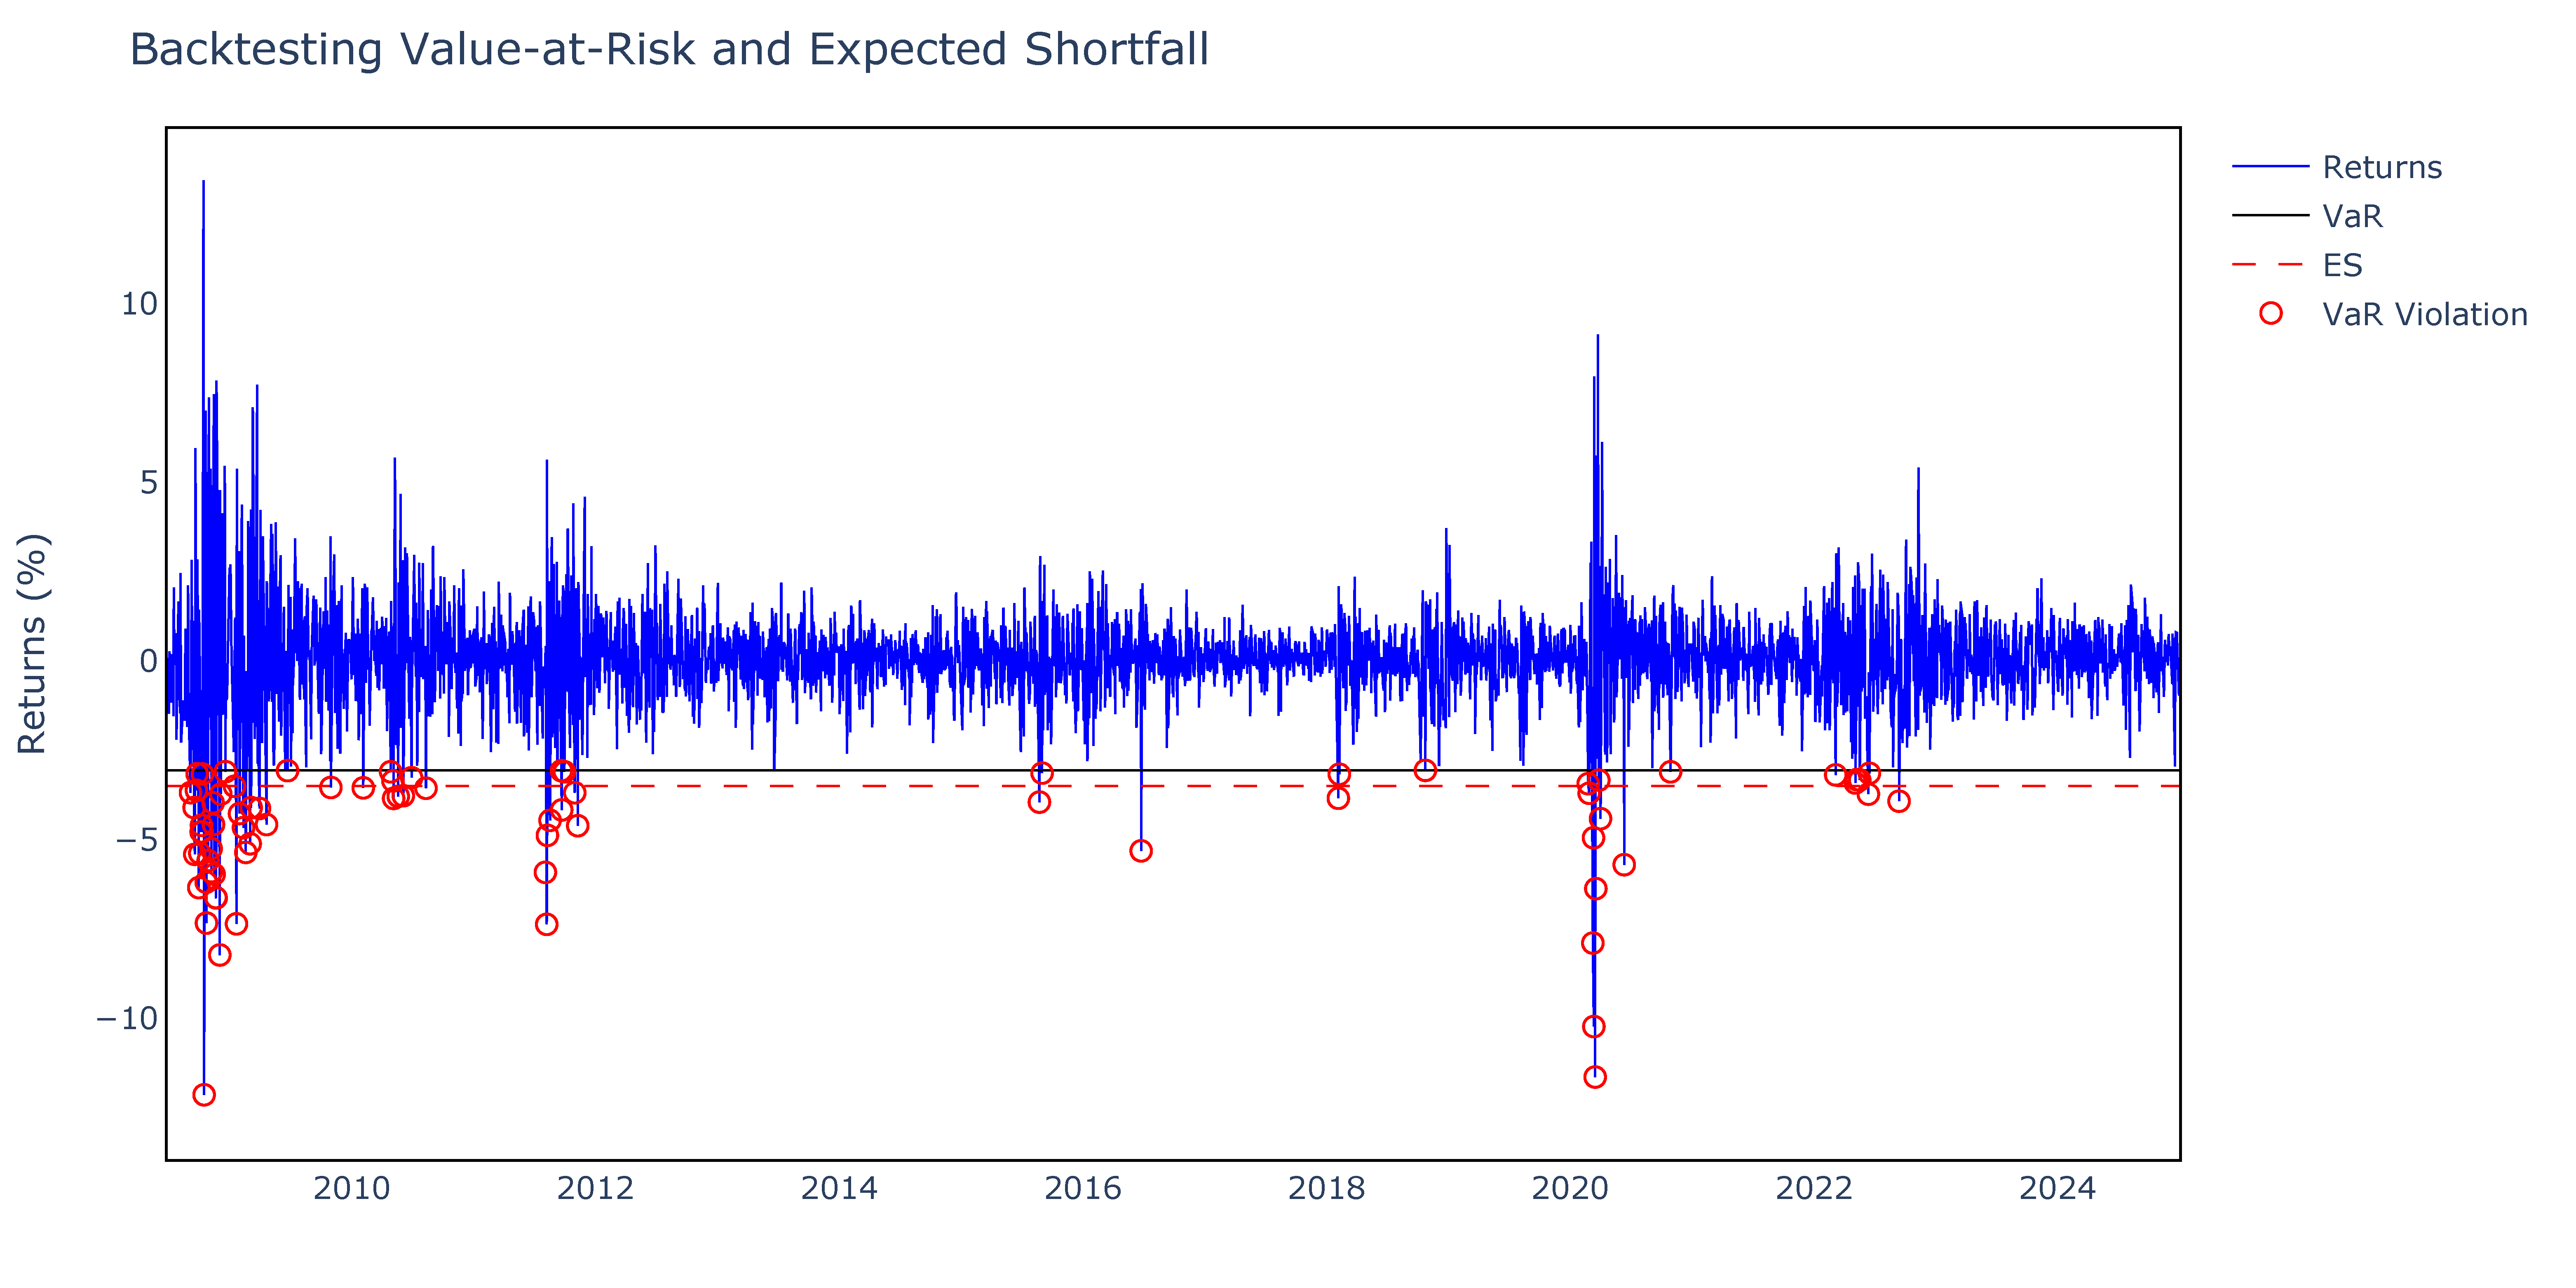
\includegraphics[width=\textwidth]{parametric_backtest.pdf}
        \caption{Backtesting results for the Parametric Normal model.}
    \end{minipage}
\end{figure}

\begin{figure}[H]
    \centering
    \begin{minipage}{0.95\textwidth}
        \centering
        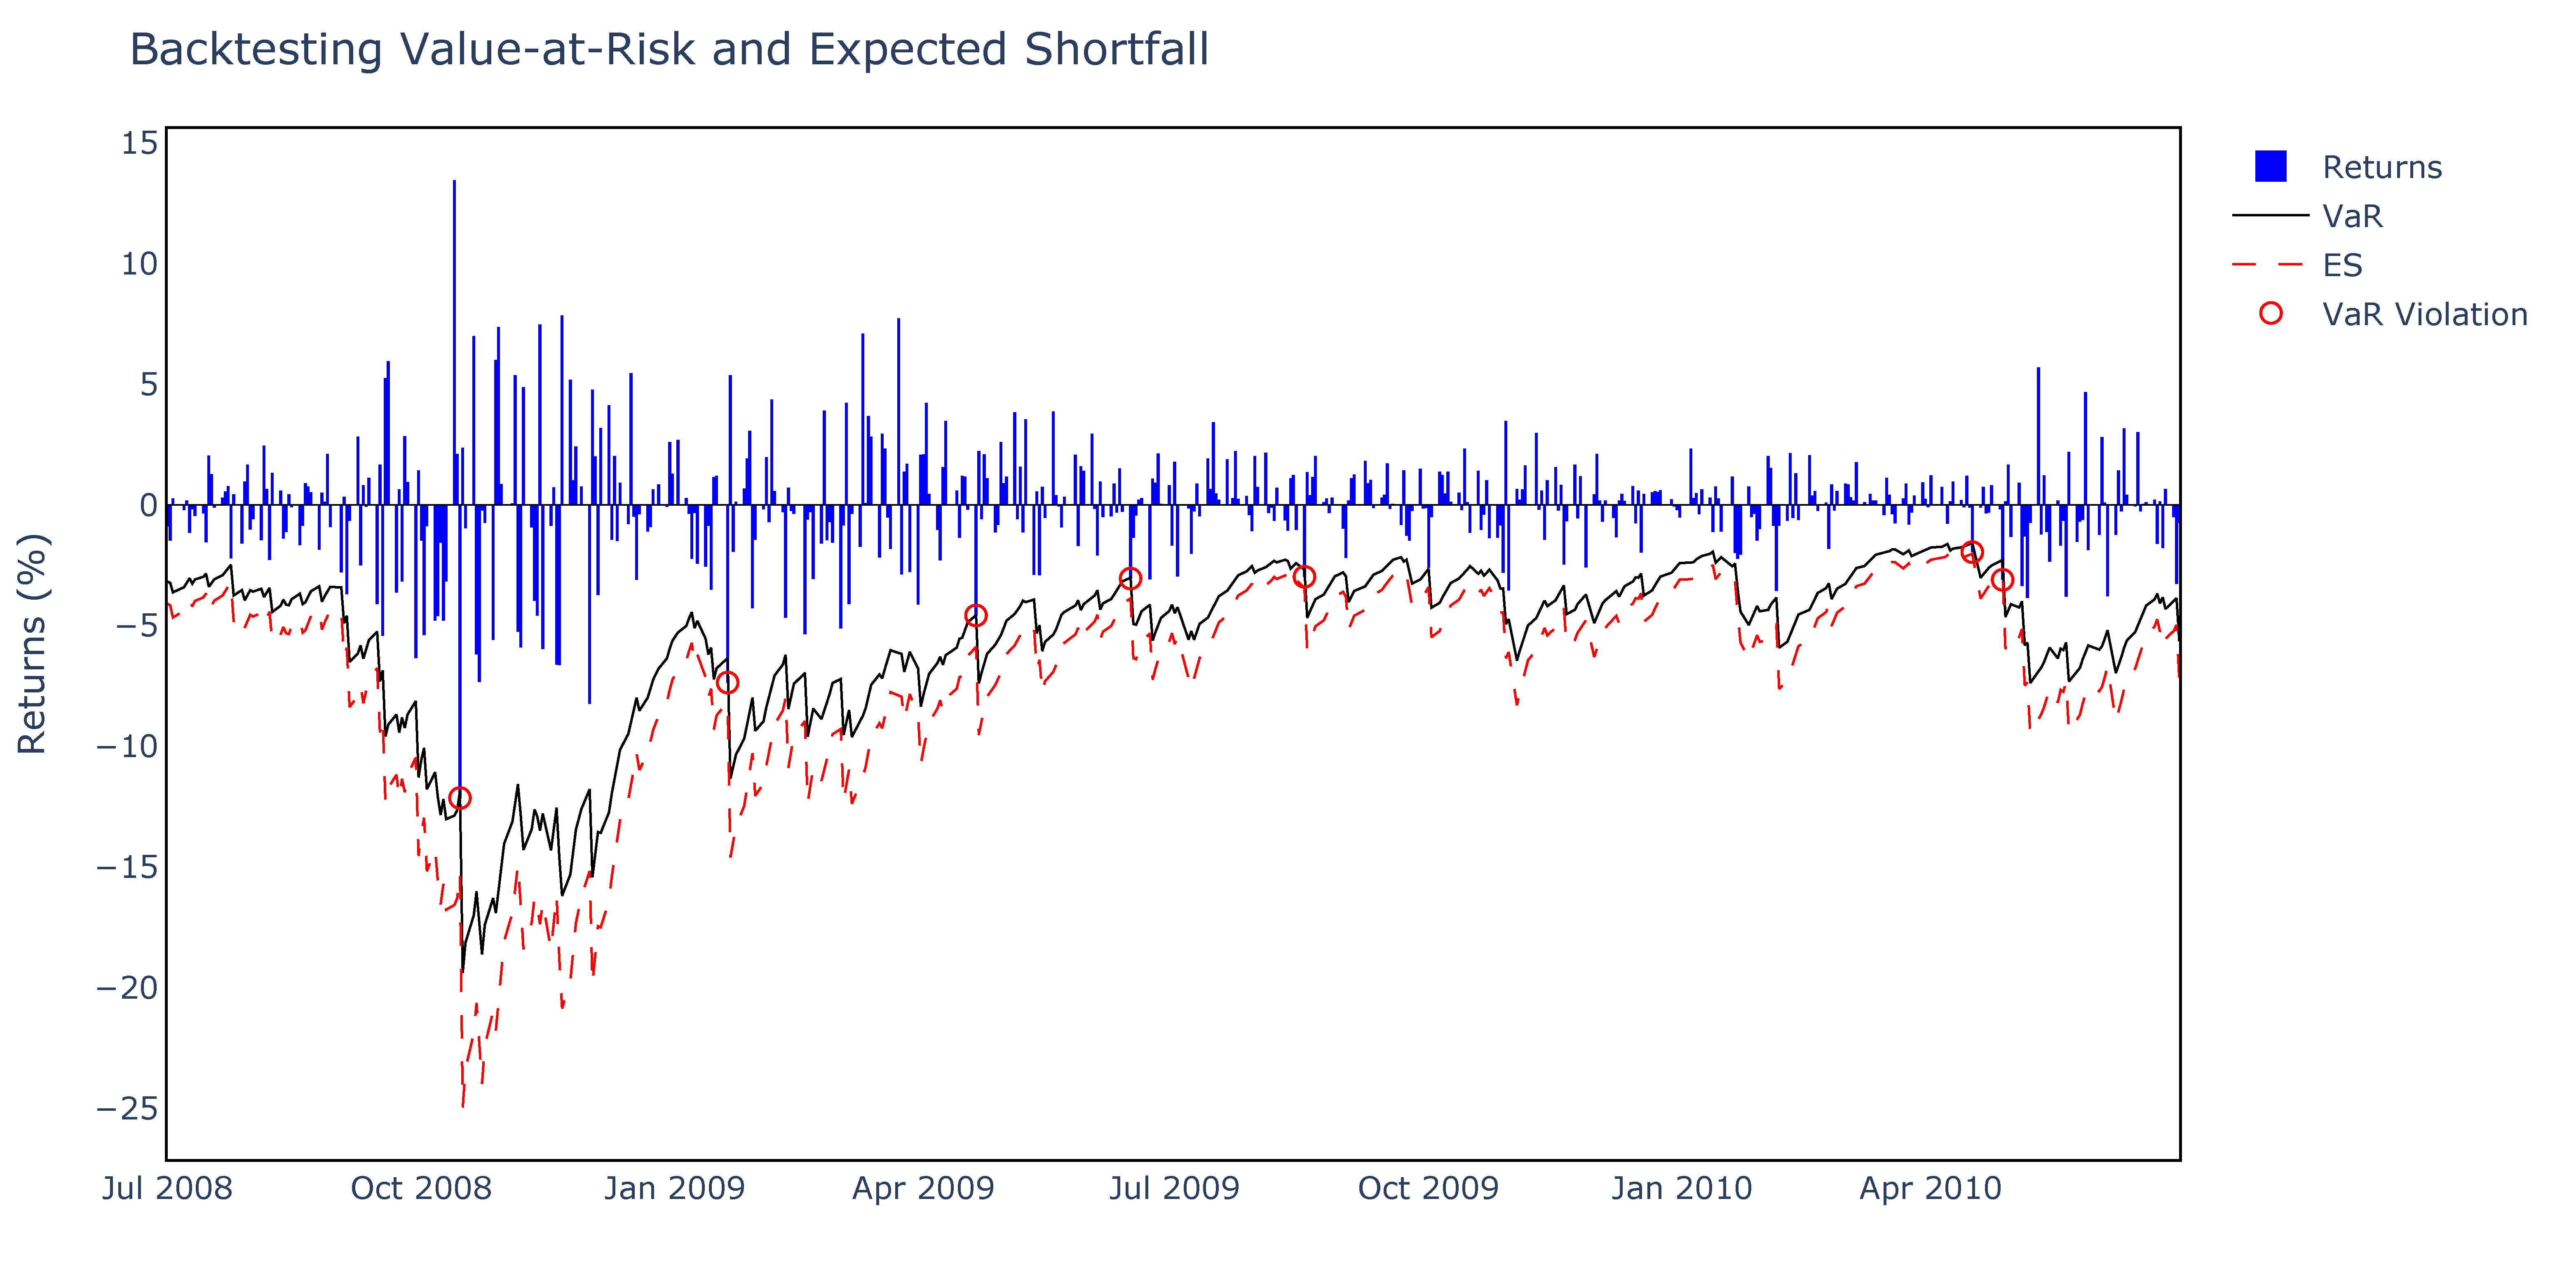
\includegraphics[width=\textwidth]{garch_backtest_subset.pdf}
        \caption{Backtesting results (subset) for the GJR-GARCH model with skewed-$t$ innovations.}
    \end{minipage}
\end{figure}

\begin{figure}[H]
    \centering
    \begin{minipage}{0.95\textwidth}
        \centering
        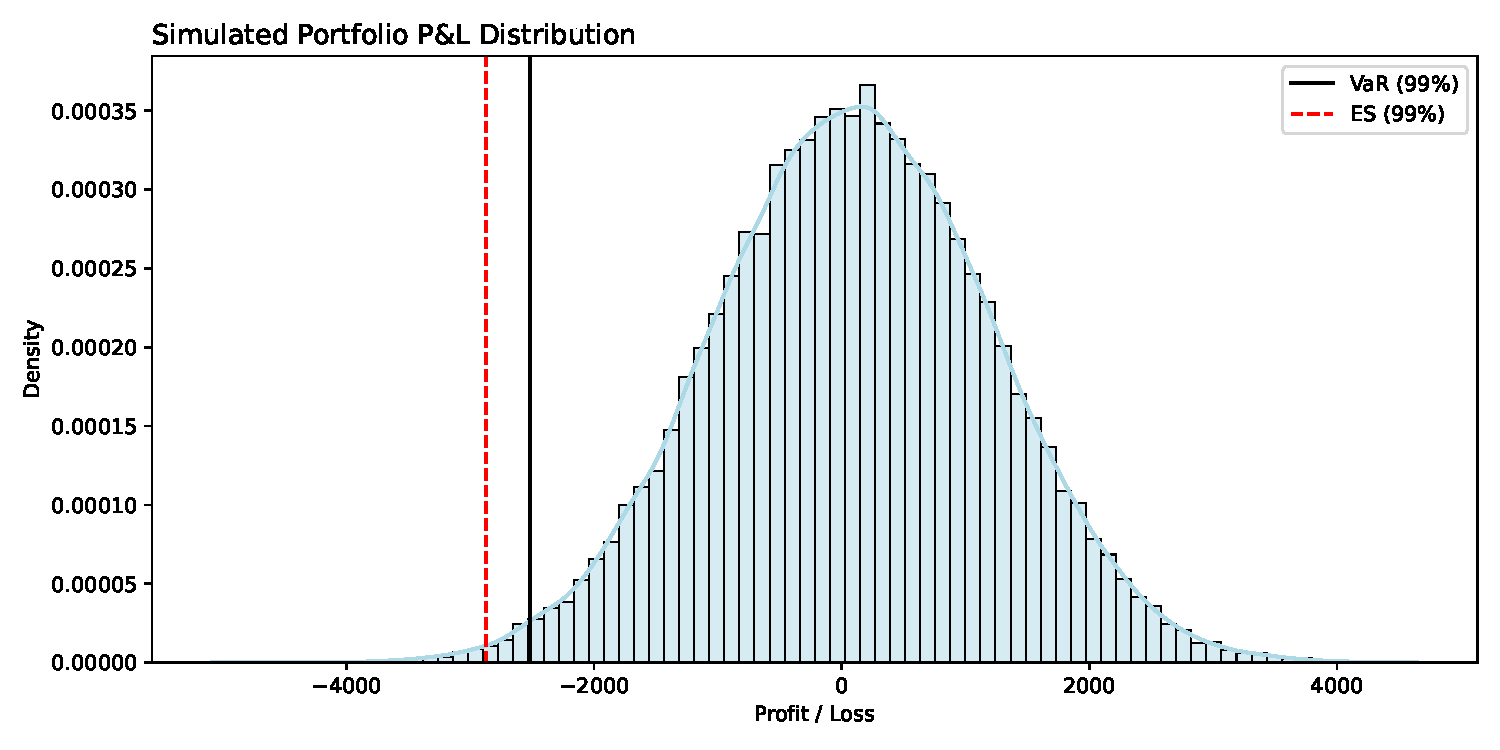
\includegraphics[width=\textwidth]{mc_simulation.pdf}
        \caption{Monte Carlo simulation results for the globally diversified portfolio.}
    \end{minipage}
\end{figure}

\begin{figure}[H]
    \centering
    \begin{minipage}{0.95\textwidth}
        \centering
        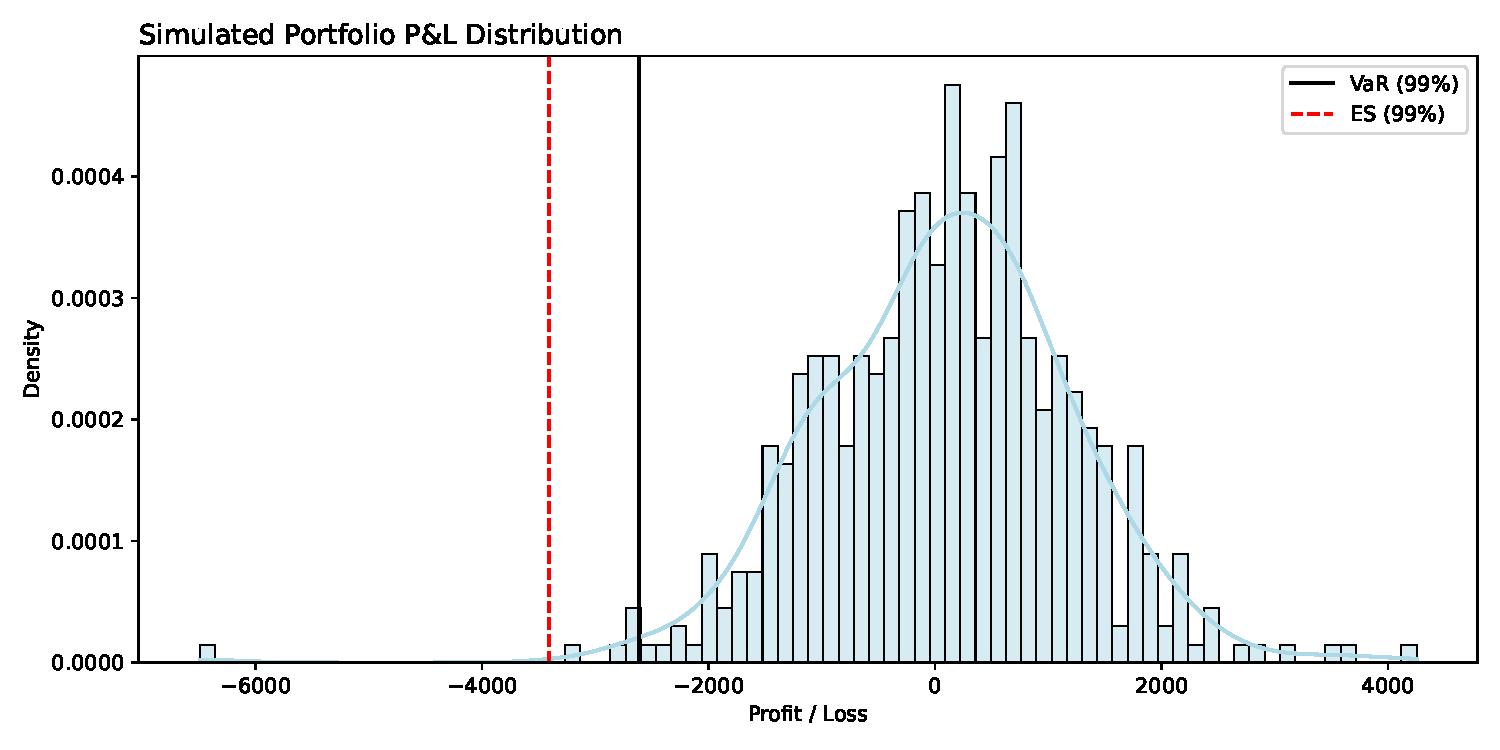
\includegraphics[width=\textwidth]{historical_simulation.pdf}
        \caption{Historical simulation results for the same portfolio.}
    \end{minipage}
\end{figure}



\end{document}

